\subsection{SIP}

The captured \gls{sip} traffic shows that it is unencrypted and the transport protocol used is \gls{udp} \cite{rfc768}. Most of the parameters to establish a connection to the \gls{voip} server of the \gls{isp} can be extracted from the traffic. Only the password is not available as plaintext and the hashed value is calculated with a nonce that makes it usable only once.

But by inspecting the configuration files and management interfaces of the \gls{cpe}s, it was possible to retrieve the plaintext \gls{sip} password. All the passwords extracted had length 16 and contained only alphanumeric characters. After further analysis, it was found that the last 8 characters of the password are always the first 8 characters with the case swapped. This pattern effectively reduces the strength of the password by a square root, so only \( 62^8 \) different passwords exist. A iterator that generates all possible passwords has been implemented and is available in Appendix \ref{appendix:sip_pwd_it}.

Running a \gls{sip} Digest Authentication benchmark with hashcat on a p3.2xlarge \gls{aws} \gls{ec2} Instance \cite{aws_ec2_p3_instances}, showed that the machine is able to brute-force the password on the captured \gls{sip} packets at a rate of 7.5 \gls{G}\gls{H}\gls{ps}, as show in Figure \ref{figure:hashcat_benchmark_sip}. It means that with an expense of no more than \$24.64, in the worst-case scenario, the weakened password can be cracked in 8h4min.

\begin{figure}[h]
    \centering
    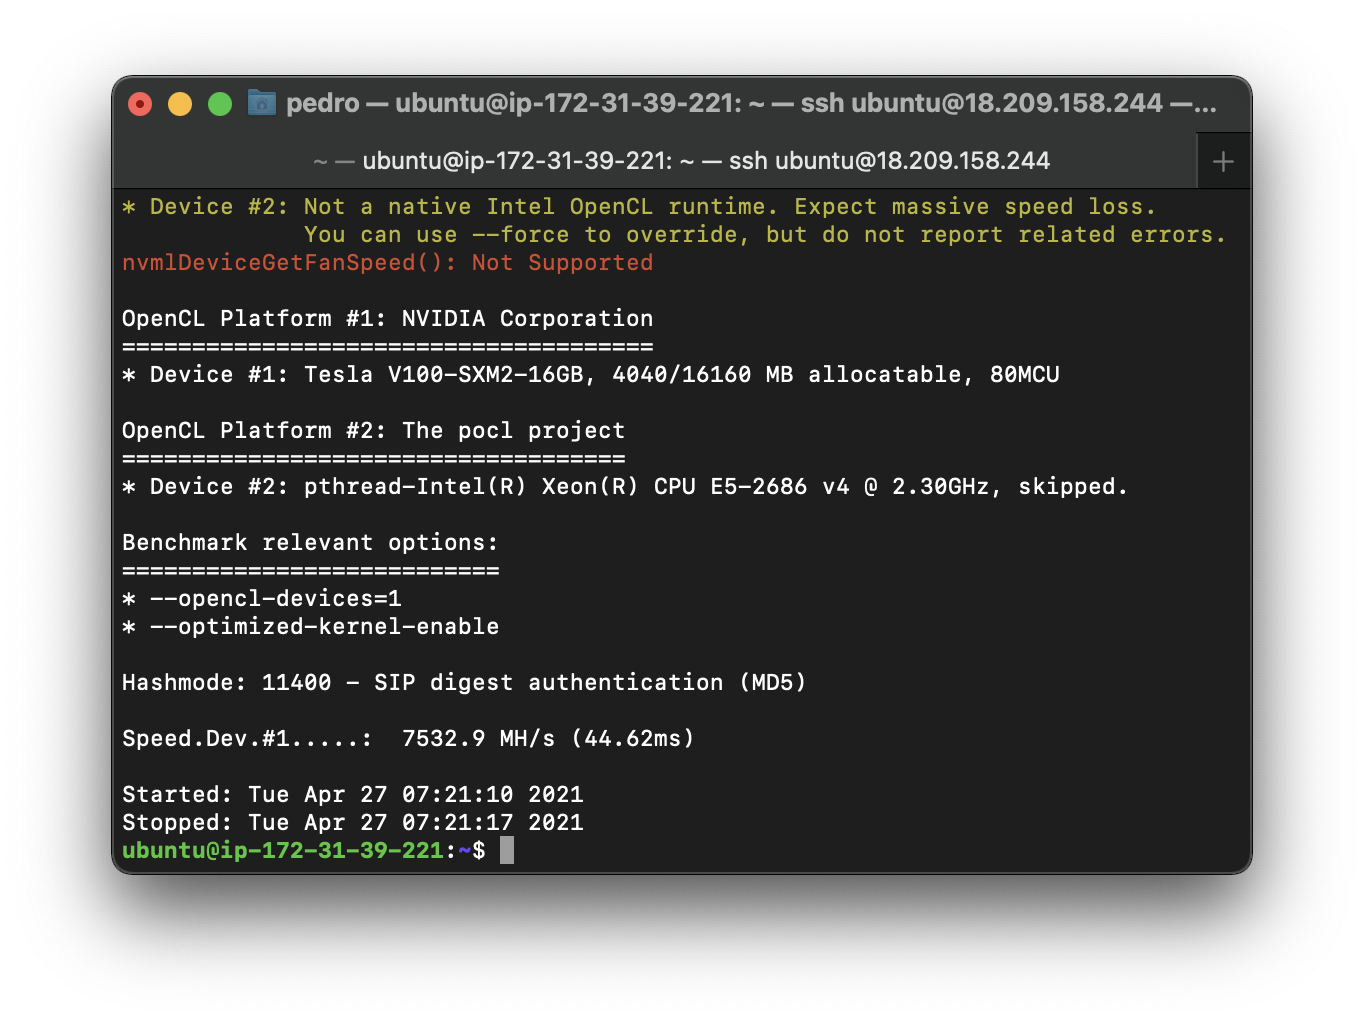
\includegraphics[width=\linewidth]{contents/configuration-analysis/sip/hashcat-benchmark-sip.png}
    \caption{Hashcat \gls{sip} Benchmark on a p3.2xlarge \gls{aws} \gls{ec2} Instance}
    \label{figure:hashcat_benchmark_sip}
\end{figure}

Enabling \gls{tls} \cite{rfc8446} would be an option to mitigate the capture of plaintext \gls{sip} requests, but it is not possible because the \gls{sip} registrar doesn’t support the encrypted protocol. Unfortunately, the customer itself is also unable to change the \gls{sip} password, only the \gls{isp} can change the password and it is unlikely that it can be set to a custom value or a value without the known pattern. Rotating the password would only mitigate an ongoing attack where the attacker has captured the hashed password but is not able to acquire it anymore. The strength is not increased and if the hash is obtained at a later point in time, it can easily be cracked again.

\FloatBarrier
